\namedchapter[Daniel Łukwiński]{Algorytm przetwarzania obrazu}
Zadanie, jakie miał realizować robot polegało na namierzeniu oraz śledzeniu celu w swoim otoczeniu. Założeniem było także to, aby algorytm robota potrafił znajdować cel przy zróżnicowanym oświetleniu oraz na różnej odległości (tj. niezależnie od jego rozmiaru na obrazie). Ważne było także, aby celem mógł być każdy obiekt spełniający podstawowe warunki koloru i kształtu. Algorytm przetwarzania i analizy obrazu ma więc za zadanie poszukiwać na dostarczanym przez kamerę obrazie celu i uzyskiwane w ten sposób informacje przesyłać do części programu odpowiedzialnej za sterowanie robotem.

\namedsection{OpenCV}
OpenCV jest biblioteką służącą do wszechstronnej obróbki obrazu, wydaną na licencji BSD (\textit{Berkeley Software Distribution}), będącej zgodną z zasadami wolnego oprogramowania. Została ona napisana w C oraz C++, jednak możliwe jest je wykorzystywanie także w językach \textit{Python} oraz \textit{Java}. Wspiera ona takie systemy operacyjne jak: \textit{Windows, Linux, Mac OS, iOS} oraz \textit{Android}. Posiada ona moduły służące do pracy tak z obrazem dwuwymiarowym, jak i trójwymiarowym. Ponadto zawiera szereg modułów, służących między innymi do rozpoznawania twarzy, gestów czy systemów uczących się (ang. \textit{machine learning}).

O jej wykorzystaniu, poza darmową licencją, zdecydowała optymalizacja zastosowanych rozwiązań oraz mnogość funkcji, spełniających większość zadań związanych z analizą obrazu. Wykorzystywana w projekcie wersja nosi oznaczenie 3.0.0 i została opublikowana 4 czerwca 2015 roku. W przedstawianym algorytmie wykorzystywane są trzy moduły z tej biblioteki:
\begin{itemize}
\item \texttt{core.hpp} - zawiera podstawowe klasy oraz funkcje związane z pracą na obrazach dwuwymiarowych;
\item \texttt{imgproc.hpp} - zawiera bardziej zaawansowane funkcje służące to przetwarzania obrazów, np.: filtrację obrazu czy progowanie;
\item \texttt{highgui.hpp} - w tym pliku znajdują się funkcje związane z interface'm programu, które zostały wykorzystane jedynie na etapie tworzenia algorytmu, do testowania jego efektów efektów (wyświetlenie obrazu, odczyt oraz zapis do pliku).
\end{itemize}

\namedsection{Inicjalizacja}
Działający na \textit{Raspberry Pi} program składa się z dwóch części. Pierwsza z nich jest odpowiedzialna za inicjalizację sprzętowych generatorów sygnału PWM na \textit{Raspberry Pi}, łączenie się z kamerą oraz rozpoczęcie jej pracy z ustalonymi parametrami.

Inicjalizacja sygnałów PWM na \textit{Raspberry Pi} jest wykonywana z wykorzystaniem biblioteki \textit{wiringPi}. Jest to napisana w języku C biblioteka obsługująca piny GPIO mini komputera \textit{Raspberry Pi}. Została ona wydana na licencji \textit{GNU LGPLv3}, umożliwiającej darmowy dostęp dla wszystkich zainteresowanych użytkowników. Pierwszym krokiem inicjalizacji sygnałów PWM jest wywołanie funkcji \texttt{int wiringPiSetupGpio()}. Znajdują się w niej deklaracje niezbędne do poprawnej pracy z biblioteką. Odpowiada ona także za umożliwienie bezpośredniego dostępu do pinów GPIO \textit{Raspberry Pi}. Wartością zwracaną przez tą funkcję jest kod, informujący o poprawności wywołania. Jego wartość równa -1 oznacza błąd uniemożliwiający dalszą prawidłową pracę. Następnie należy wywołać funkcję \textit{void pinMode (int pin, int mode)}, której zadaniem jest ustawienie jednego z pinów GPIO Rasppbery w odpowiedni tryb: wejścia, wyjścia, wyjścia zegara lub wyjścia sygnału PWM. W tym przypadku koniecznie jest ustawienie pinów numer 18 oraz 19 jako wyjścia sygnału PWM. Kolejną wywoływaną funkcją z tej biblioteki jest void \texttt{pwmSetMode(int mode)}. Ma ona za zadanie ustalić w którym z dwóch trybów ma pracować generator sygnału PWM: \textit{mark:space} lub \textit{balanced}. Pierwszy z nich jest klasycznym sygnałem PWM, w którym okres sygnału jest równy całemu cyklowi pracy licznika. W drugim wartość wypełnienia jest równomiernie rozłożona na cykl licznika, przez co wyjściowa częstotliwość sygnału jest dużo większa. W zastosowanym algorytmie wykorzystany został pierwszy tryb, gdyż dużo lepiej nadaje się on do sterowania serwomechanizmów. Kolejne dwa niezbędne do ustawienia parametry to zakres licznika oraz preskaler zegara. Wykorzystuje się do tego dwie funkcje: \texttt{void pwmSetRange (unsigned int range)} oraz \texttt{void pwmSetClock (int divisor)}. Wpływ tych dwóch parametrów przedstawia wzór:
\begin{equation}
f_{PWM} = \frac{f_{count}}{range} = \frac{f}{(divisor * range)}
\label{eq:hard_pwm}
\end{equation}
gdzie:
\begin{equationDescriptor}
\EQDitem{$f_{PWM}$}{częstotliwość sygnału PWM [$Hz$],}
\EQDitem{$f_{count}$}{częstotliwość pracy licznika [$Hz$],}
\EQDitem{$f$}{częstotliwość zegara bazowego [$Hz$],}
\EQDitem{$divisor$}{Wartość preskalera,}
\EQDitem{$range$}{Zasięg licznika, }
\end{equationDescriptor}
W przypadku zastosowanych serwomechanizmów wymagane $f_{PWM}$ wynosi 50 $Hz$, a $f$ dla \textit{Raspberry Pi} to 19.2 $MHz$. Przedstawiony wcześniej wzór przyjmuje więc postać:
\begin{equation}
50 Hz = \frac{19.2 MHz}{(divisor * range)}
\label{eq:hard_pwmN}
\end{equation}
Widać więc jasno, że wartość preskalera oraz zasięg liczniki są ze sobą powiązane i muszą być ustawiane wspólnie, a wartość ich iloczynu wynosi:
\begin{equation}
(divisor * range) = \frac{19.2 MHz}{50 Hz} = 384000
\label{eq:range_x_presc}
\end{equation}
O dokładności sterowania serwomechanizmem decyduje właśnie wartość zasięgu licznika służącego do generowania sygnału PWM. Wspomniane wcześniej funkcje z biblioteki \textit{WiringPi} służące do ustawiania tych dwóch parametrów przyjmują tylko wartości całkowite, więc wybierany zasięg licznika powinien być dzielnikiem liczby $384000$. Wartość zasięgu ustawiono więc na poziomie 6000, co zapewnia wystarczającą dokładność pracy serwomechanizmu, a to z kolei pociągnęło za sobą ustawienie preskalera zegara na 64. Ostatecznie blok kodu odpowiedzialny na inicjalizację sprzętowego generatora sygnału PWM w \textit{Raspberry Pi} za pomocą biblioteki \textit{WiringPi} przyjmuje postać:
\begin{lstlisting}[caption=Inicjalizacja sygnałów PWM \textit{Raspberry Pi}]
if (wiringPiSetupGpio() != -1)
{
	pinMode(18,PWM_OUTPUT);
	pinMode(19,PWM_OUTPUT);
	pwmSetMode(PWM_MODE_MS);
	pwmSetRange(6000);
	pwmSetClock(64)
}
else
{
	return -1;
}
\end{lstlisting}

Drugą rzeczą, obok sygnału PWM, wymagającą inicjalizacji na początku pracy programu jest kamera. Do jej obsługi wykorzystana została biblioteka \textit{RaspiCamCV}, udostępniana na zasadach wolnego oprogramowania. Została ona wybrana, ponieważ zapewnia podstawową obsługę dedykowanej kamery \textit{Raspberry Pi} we współpracy z biblioteką \textit{OpenCV}. Z jej wykorzystaniem możliwe jest pobieranie rejestrowanych obrazów bezpośrednio w formacie umożliwiającym dalszą edycję za pomocą funkcji \textit{OpenCV}. Pierwszym etapem pracy z dedykowaną kamerą, z wykorzystaniem biblioteki \textit{RaspiCamCV}, jest utworzenie danych konfiguracyjnych, które posłużą do ustawienia parametrów pracy kamery. Podstawowym ustawieniem, które należy wybrać jest rozdzielczość w jakiej będą rejestrowane obrazy. Jest to o tyle istotne, że podstawowym ograniczeniem w pracach nad algorytmem wykrywającym cel był fakt, że wyniki jego pracy miały na bieżąco sterować ruchami pojazdu, przy ograniczonej mocy obliczeniowej platformy \textit{Raspberry Pi}. Podstawowym ograniczeniem, które spowodowały te warunki, była rozdzielczość analizowanego obrazu. Oferowana przez kamerę rozdzielczość maksymalna wynosi aż 1920 na 1080 pikseli, jednak jest to o wiele za dużo, jak na stawiane przed algorytmem wymagania. Ostatecznie zdecydowano się wykorzystać rozdzielczość 640 na 480 pikseli. Taki rozmiar zapewnia jeszcze zadowalający poziom dokładności zdjęcia oraz relatywnie szybką jego analizę. Pozostałe parametry zostały ustawione na wartości domyślne, ponieważ wtedy są one samoczynnie dobierane na podstawie warunków pracy, co zapewniło zdjęcia bardzo dobrej jakości nawet przy zróżnicowanym oświetleniu.

Po stworzeniu danych konfiguracyjnych pozostało utworzyć obiekt (a właściwie wskaźnik na taki obiekt), który w trakcie pracy programu będzie służył do pobierania ostatniego wykonanego przez kamerę zdjęcia znajdującego się w buforze. Całość kodu wykorzystywanego do inicjalizacji pracy kamery przedstawia się w sposób następujący:
\begin{lstlisting}[caption=Inicjalizacja pracy kamery]
RASPIVID_CONFIG* config = (RASPIVID_CONFIG*)malloc(sizeof(RASPIVID_CONFIG));
config->width = 640;
config->height = 480;
config->bitrate = 0;
config->framerate = 0;
config->monochrome = 0;
RaspiCamCvCapture* capture =
	(RaspiCamCvCapture *)raspiCamCvCreateCameraCapture2(0, config);
free(config); 
\end{lstlisting}

\namedsection{Przetwarzanie obrazu}
Po fazie inicjalizacji program rozpoczyna pracę w nieskończonej pętli. Można ją podzielić na dwa etapy: analiza obrazu oraz wysłanie sygnałów sterujących na jej podstawie. Jak wspomniano na początku rozdziału poszukiwanym na obrazie celem ma być czerwone koło. Wymaga to analizy obrazu w dwóch płaszczyznach: koloru oraz geometrii. W pierwszej kolejności obraz będzie przetwarzany pod kątem wyodrębnienia jedynie obiektów czerwonych, a następnie wśród nich poszukiwany będzie okrąg.

Pierwszy etap pętli rozpoczyna na się od pobrania najnowszego wykonanego przez kamerę zdjęcia. Korzystając z funkcji biblioteki \textit{RaspiCamCV} możliwe jest uzyskanie obrazu wspieranego już przez \textit{OpenCV}. Dzięki temu możliwe jest bezpośrednie przejście do jego przetwarzania.

Dalsza część algorytmu poświęcona jest wyodrębnieniu czerwonych obiektów. Wybór akurat tego koloru o tyle ułatwia zadanie, że możliwe jest pozostanie przy omówionym wcześniej modelu RGB, w którym jedna z trzech składowych obrazu odpowiada za ten właśnie kolor. Pierwszą wykonywaną operacją jest więc rozłożenie otrzymanego z kamery obrazu w formacie RGB na trzy osobne macierze za pomocą funkcji \texttt{split} z biblioteki \textit{OpenCV}. Należy jednak pamiętać, że kolor czerwony jest także składową wielu innych barw, co dobrze przedstawia ilustracja \ref{red}.
\begin{figure}[H]
\begin{center}
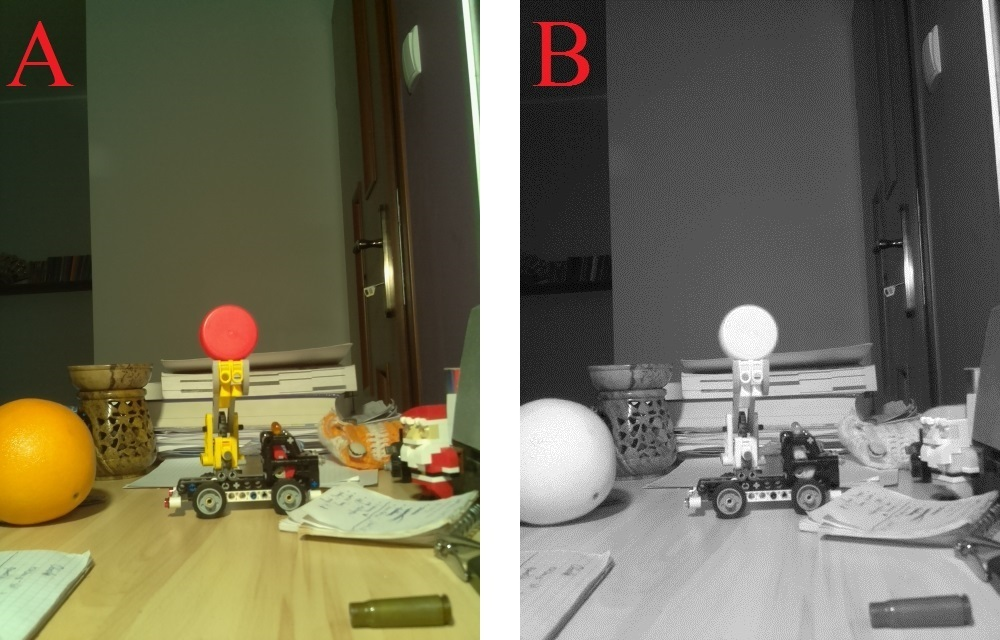
\includegraphics[scale=0.42]{imgs/imgBase+Red.jpg}
\caption[Uzyskany kanał czerwony wraz z oryginalny obrazem.]\small{A - oryginalne zdjęcie wykonane przez kamerę \textit{Raspberry Pi}, B - kanał czerwony tego zdjęcia.}
\label{red}
\end{center}
\end{figure}
Analizując jedynie prawe zdjęcie, przedstawiające intensywność koloru czerwonego, nie sposób oddzielić barwy czerwonej od tych, w których skład wchodzi kolor czerwony. Konieczna jest dalsze przetwarzanie danego obrazu.

W przedstawianym algorytmie zdecydowano się na wyszczególnienie obiektów o kolorze czerwonym poprzez usunięcie z kanału czerwonego barw, w których czerwień jest tylko mniej istotną składową. Każdy z kanałów obrazu: czerwony, zielony czy niebieski są dwuwymiarowymi macierzami o wartościach całkowitych z przedziału od 0 do 255. Odejmowanie ich od siebie nawzajem polega więc na odjęciu od siebie dwóch macierzy o jednakowych wymiarach. Operację taką przedstawia równanie:
\begin{equation}
c_{i,j} = a_{i,j} - b_{i,j}, \text{	dla	} i \in N, j \in M
\label{eq:odejmowanie}
\end{equation}
gdzie:
\begin{equationDescriptor}
\EQDitem{$c_{i,j}$}{element macierzy $C$ o współrzędnych $i$ oraz $j$,}
\EQDitem{$a_{i,j}$}{element macierzy $A$ o współrzędnych $i$ oraz $j$,}
\EQDitem{$b_{i,j}$}{element macierzy $B$ o współrzędnych $i$ oraz $j$,}
\EQDitem{$N$}{liczba wierszy,}
\EQDitem{$M$}{liczba kolumn.}
\end{equationDescriptor}
Należy jednak pamiętać, że wartość każdego piksela musi zawierać się w przedziale od 0 do 255. Do takiego poziomu więc ograniczane są wartości w macierzy wynikowej:
\begin{equation}
c_{i,j} =
  \begin{cases}
    c_{i,j}	& \quad \text{dla } 0 \leq c_{i,j} \leq 255\\
    0	& \quad \text{dla } c_{i,j} < 0\\
    255	& \quad \text{dla } c_{i,j} > 255\\
  \end{cases}
\label{eq:progowanie}
\end{equation}
gdzie:
\begin{equationDescriptor}
\EQDitem{$c_{i,j}$}{element macierzy $C$ o współrzędnych $i$ oraz $j$.}
\end{equationDescriptor}
Usunięcie z kanału czerwonego obszarów, w których czerwień jest tylko mniej istotną składową, odbywa się poprzez proste odjęcie od barwy czerwonej barw zielonej oraz niebieskiej. Powoduje to jednak zbyt duże podkreślenie różnic między obszarami o różnym oświetleniu. Sytuację taką prezentuje ilustracja \ref{red-b+g}. Widać na niej, że nawet na jednorodnych obiektach powstają bardzo duże różnice w jasności, zależne od padającego na obiekt światła. Dzieje się tak, ponieważ mocniejsze oświetlenie piksela podnosi poziom jego wartości we wszystkich trzech macierzach RGB.\newpage
\begin{figure}[H]
\begin{center}
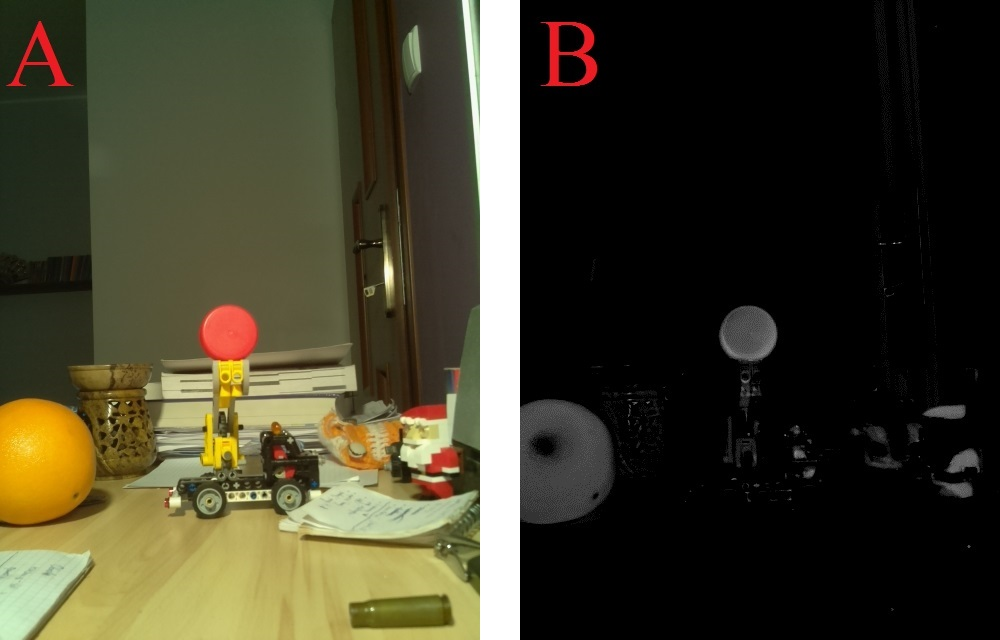
\includegraphics[scale=0.42]{imgs/imgBase+sumBG.jpg}
\caption[Kanał czerwony minus zielony oraz niebieski.]\small{A - przedstawiony dla porównania oryginalny obraz, B - obraz powstały z odjęcia od kanału czerwone sumy kanałów zielonego oraz niebieskiego.}
\label{red-b+g}
\end{center}
\end{figure}
Sytuacja taka może prowadzić do wielu nieprawidłowości w zachowaniu algorytmu, więc należało zastosować inną metodę wyszczególniania czerwonej barwy. Zamiast odejmowania sumy kanałów zielonego i niebieskiego zdecydowano się na wyznaczanie macierzy wartości maksymalnej tych dwóch barw i odjęcie jej od kanału czerwonego. Operacja ta powoduje dużo mniejsze zróżnicowanie obrazu końcowego, który jest także mniej wrażliwy na zróżnicowane oświetlenie. Wyznaczenie maksimum dwóch macierzy polega na wpisaniu do macierzy wynikowej wartości większej z porównywanych macierzy wejściowych. Prezentuje to poniższy wzór:
\begin{equation}
c_{i,j} =
  \begin{cases}
    a_{i,j}	& \quad \text{dla } a_{i,j} \geq b_{i,j}\\
    b_{i,j}	& \quad \text{dla } a_{i,j} < b_{i,j}\\
  \end{cases}
\label{eq:progowanie}
\end{equation}
gdzie:
\begin{equationDescriptor}
\EQDitem{$c_{i,j}$}{element macierzy $C$ o współrzędnych $i$ oraz $j$,}
\EQDitem{$a_{i,j}$}{element macierzy $A$ o współrzędnych $i$ oraz $j$,}
\EQDitem{$b_{i,j}$}{element macierzy $B$ o współrzędnych $i$ oraz $j$.}
\end{equationDescriptor}
Wynik operacji wyznaczającej maksimum kanału zielonego i niebieskiego oraz odjęcie go od kanału czerwonego przedstawia rysunek \ref{red-max}.\newpage
\begin{figure}[H]
\begin{center}
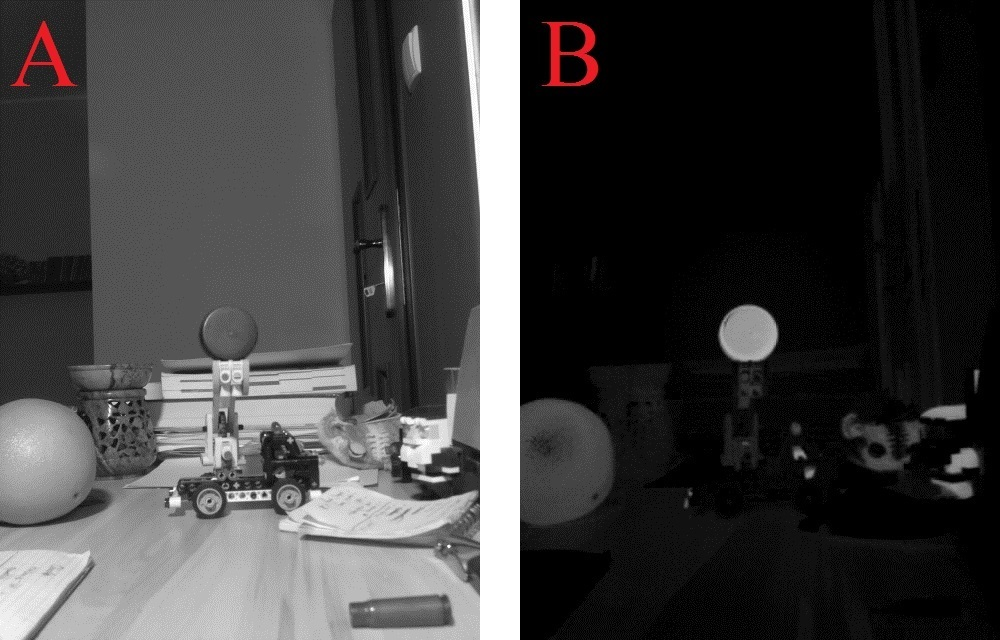
\includegraphics[scale=0.42]{imgs/imgMax+RwoBG.jpg}
\caption[Kanał czerwony minus maksimum zielonego i niebieskiego.]\small{A - obraz powstały jako maksimum kanałów zielonego i niebieskiego, B - wynik odjęcia wspomnianego maksimum od kanału czerwonego.}
\label{red-max}
\end{center}
\end{figure}
Jak widać, poza bardziej jednolitym przedstawieniem jednorodnych obiektów, udało się uzyskać bardziej wyróżniający się kolor czerwony w stosunku do np. pomarańczowego.

Odejmowanie od siebie zróżnicowanych obrazów może powodować jednak powstanie dużych różnic jasności blisko położonych pikseli.  Efekt ten powoduje na dalszych etapach analizy obrazu problemy z odnajdywaniem regularnych geometrycznych kształtów, co sprowadza się do trudności z wykrywaniem okręgów. Problem ten rozwiązuje zastosowanie filtru medianowego na macierzy maksimów koloru niebieskiego i zielonego.

Filtr medianowy jest narzędziem wykorzystujący jedną z podstawowych wartości statystycznych jaką jest mediana. Polega ona na wyznaczaniu środkowego elementu w monotoniczne uporządkowanym ciągu\cite{Malina}. W przypadku filtru medianowego ciągiem tym jest zbiór pikseli, który na obrazie pokrywa maska filtru. Przykłady stosowanych masek przedstawia ilustracja \ref{maski}. Element zaznaczony na niej jako ,,X", jest elementem do którego wpisany zostanie wynik mediany.\newpage
\begin{figure}[H]
\begin{center}
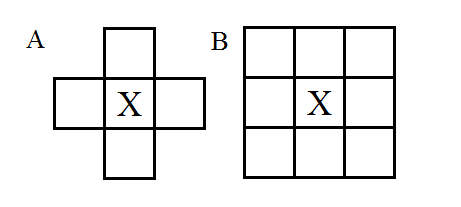
\includegraphics[scale=0.8]{imgs/maski.png}
\caption[Przykład masek filtru medianowego.]\small{Przykład masek wykorzystywanych w filtrze medianowym: A - maska 5-elementowa, B - maska 9-elementowa. Znakiem ,,X" oznaczono element docelowy wyniku mediany.}
\label{maski}
\end{center}
\end{figure}
Filtr ten ujednolica obraz, usuwając z niego piksele o wartościach skrajnych. Ponadto cechą charakterystyczną jest także to, iż zaokrągla on znajdujące się na obrazie kształty. Obie te cechy czynią z tego filtru bardzo użyteczne narzędzie w przedstawianym algorytmie, gdyż wyrównują one poszukiwane geometryczne regularności na obrazie, które wskutek przekształceń oraz niewielkiej rozdzielczości mogą zostać zniekształcone. Wykorzystywana w tym miejscu algorytmu maska ma kształt kwadratu oraz wymiarach 5 na 5 pikseli. Efekt jej działania przedstawia ilustracja \ref{red-maxM}, na której widać obraz będący maksimum kanału zielonego i niebieskiego po filtracji medianowej oraz wynik odejmowania od kanału czerwonego wspomnianego maksimum. Są to te same obrazy co na ilustracji \ref{red-maxM}, różniące się jedynie zastosowaniem filtracji.
\begin{figure}[H]
\begin{center}
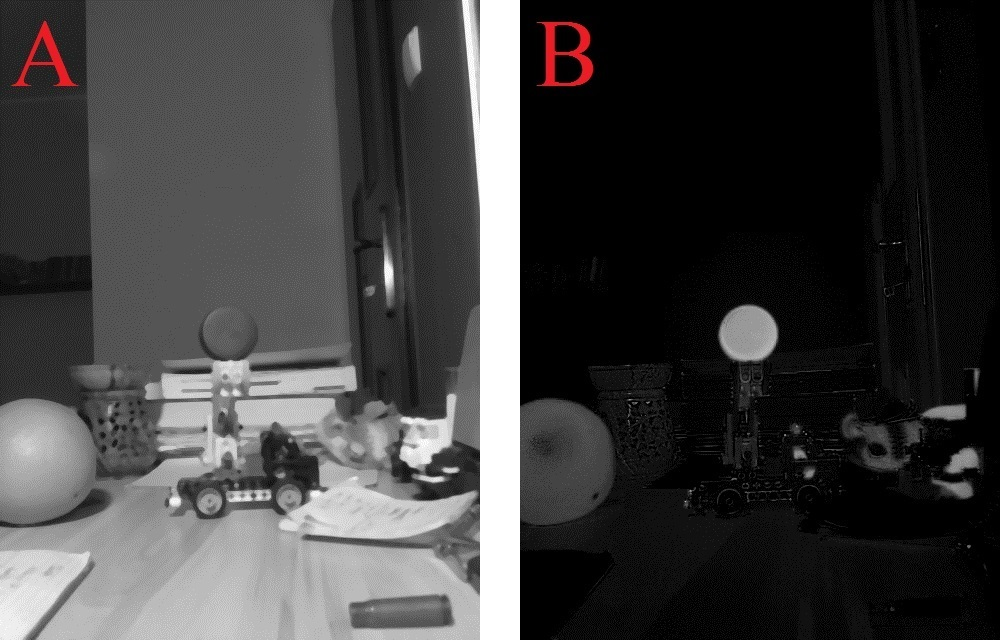
\includegraphics[scale=0.42]{imgs/imgMax+RwoBG_med.jpg}
\caption[Kanał czerwony po odjęciu maksimum kanału zielonego i niebieskiego z filtrem medianowym.]\small{A - obraz powstały jako maksimum kanałów zielonego i niebieskiego oraz z filtrem medianowym, B - wynik odjęcia wspomnianego maksimum od kanału czerwonego.}
\label{red-maxM}
\end{center}
\end{figure}
Porównując obrazy B z ilustracji \ref{red-max} i \ref{red-maxM} widać oczekiwany efekt działania filtru. Krawędzie są bardziej dokładnie, a same obiekty posiadają bardziej jednolity poziom jasności.

Na tym etapie udało się uzyskać obraz z wyróżnionymi obszarami czerwonego koloru o dużym poziomie szczegółowości. Kolejny etap algorytmu zakłada podzielenie obrazu na obszary z wyróżniającym się kolorem czerwonym oraz na pozostałe, nie zawierające istotnych informacji. Operacja, polegająca na podzieleniu obrazu na obszary, posiadające pewne cechy wyróżniające je od sąsiedztwa nazywana jest segmentacją\cite{Malina}. Jedną z podstawowych metod segmentacji, wykorzystaną także w tym przypadku, jest progowanie binarne. Polega ono na porównaniu każdego piksela z pewną wartością progową i, w zależności od wyniku porównania, przypisaniu mu jednego z dwóch poziomów jasności. Do wykonania tej operacji wykorzystywana została funkcja \textit{cvThreshold} z biblioteki \textit{OpenCV}. Do każdego pikseli poniżej wartości progu przypisuje ona poziom 0, z kolei tym przekraczającym próg pewną ustalaną przy jej wywoływaniu wartość. Działanie tego typu progowania można przedstawić za pomocą wzoru \ref{eq:progowanie}.
\begin{equation}
J_p(x, y) =
  \begin{cases}
    0	& \quad \text{dla } J(x, y) < t\\
    b	& \quad \text{dla } J(x, y) \geq t\\
  \end{cases}
\label{eq:progowanie}
\end{equation}
gdzie:
\begin{equationDescriptor}
\EQDitem{$J_p(x, y)$}{wartość piksela po progowaniu,}
\EQDitem{$J(x, y)$}{wartość piksela przed progowaniem,}
\EQDitem{$t$}{wybrany próg,}
\EQDitem{$b$}{wartość przypisana do piksela w sytuacji, gdy jego poziom jasności przed progowaniem przekroczył próg.}
\end{equationDescriptor}
W przedstawianym algorytmie wartość progu została uzależniona od jasności samego obrazu, aby uzyskać poprawne działanie algorytmu przy różnych rodzajach oświetlenia otoczenia robota. Zdecydowano się na wartość wynoszącą 0.75 poziomu najjaśniejszego piksela występującego na obrazie, co jest wartością dobraną na podstawie obserwacji wykonanych obrazów. Kolejnym koniecznym do ustalenia parametrem jest poziom jasności piksela w sytuacji, gdy przekroczył on próg. Nie jest ona tutaj aż tak istotnym parametrem i ustawiona została na poziomie 255, czyli maksimum dla przetwarzanego obrazu 8-bitowego. Efektem tak przeprowadzonego progowania jest czarno-biały obraz, na którym obiekty wyróżniające się czerwoną barwą przedstawione są białym kolorem, pozostały obszar jest czarny.

Operacja progowania wykonywana na obrazie z pełną skalą szarości, przy pomocy stałego progu, może jednak powodować utratę części geometrii. Przykładowo w sytuacji, gdy krawędź czerwonego okręgu znajduje się w cieniu jego pozostałej części to istnieje ryzyko jej odcięcia. W omawianym programie, przed takimi sytuacjami, chroni ponowne wykorzystanie filtru medianowego, tym razem z zastosowaniem maski kwadratowej o wymiarach 13 na 13 pikseli. Wspomniane wcześniej efekty, tj. wygładzanie krawędzi oraz wyrównywanie poziomu jasności bardzo dobrze nadaje się do przygotowania obrazu do operacji progowania, które ma za zadanie zachować regularne, geometryczne kształty. Porównanie obrazów przed i po progowaniu, z i bez filtru medianowego przedstawia ilustracja \ref{threshold}.
\begin{figure}[H]
\begin{center}
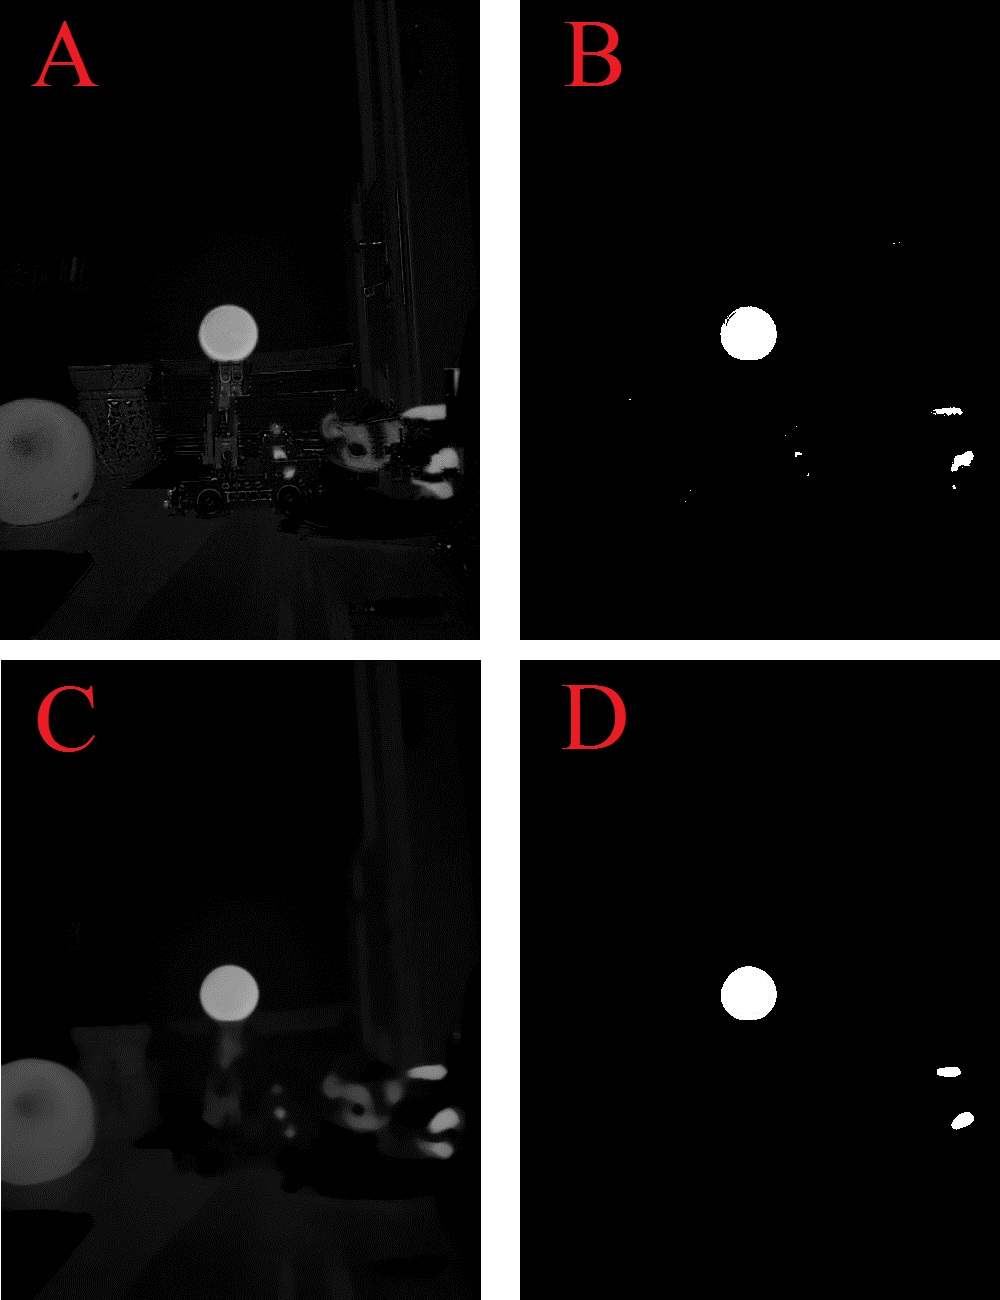
\includegraphics[scale=0.6]{imgs/img_prog+med.jpg}
\caption[Efekt progowania z oraz bez filtru medianowego.]\small{A - obraz początkowy bez zastosowanego filtru medianowego, B - efektem progowania bez wcześniejszego zastosowania filtru medianowego, C - obraz początkowy na którym zastosowano filtr medianowy, D - efekt operacji progowania po wcześniejszym zastosowaniu filtru medianowego.}
\label{threshold}
\end{center}
\end{figure}
Na przedstawionych zdjęciach A oraz C widoczny jest efekt tworzenia obszarów jednolitego koloru na obrazie. Duże obiekty stały się bardziej regularne, za to mniejsze szczegóły uległy zamazaniu. Efekty wykorzystania filtru są także widoczne na obrazach B oraz D, będących efektem progowania. Zachowane białe obszary, reprezentujące czerwone obiekty na oryginalnym zdjęciu, posiadają bardziej regularne krawędzie, zniknęły także ubytki wewnątrz figur oraz pojedyncze białe piksele widoczne w różnych miejscach obrazu B.

\namedsection{Analiza obrazu}
Efektem przetwarzania uzyskanego z kamery zdjęcia jest binarny obraz, który zostaje następnie poddany analizie, mającej za zadanie znaleźć występujące na nim okręgi. Do tego celu wykorzystana została transformacja Hougha. Jej podstawowa wersja została opracowana przez Paula Hougha w 1962 roku i służyła do detekcji linii prostych. Z czasem metodę tę jednak rozwijano, uogólniając o inne, dające się opisać analitycznie, kształty. Jej wariacja służąca do detekcji okręgów została przedstawiona w 1972 przez Richarda Duda oraz Petera Harta.

Zasada działania algorytmu Hougha opiera się na budowie macierzy zwanej akumulatorem, której liczba wymiarów jest równa liczbie zmiennych w funkcji szukanego obiektu. Z kolei rozmiary tej macierzy mówią o tym, jak wiele wartości dany parametr obiektu może przyjmować. Każdy punkt akumulatora odpowiada więc jednemu konkretnemu obiektowi znajdującemu się na obrazie. W trakcie realizowania transformaty Hougha wartość danej pozycji akumulatora jest inkrementowana dla każdego punktu na obrazie, który może należeć do obiektu definiowanego przez tą pozycję. Po przeanalizowaniu w ten sposób całego obrazu wybiera się, zgodnie z założonym wcześniej progiem, maksima w macierzy akumulatora, których współrzędne są parametrami znalezionych obiektów\cite{Sonka}.

Obiekt szukany w przedstawianym algorytmie jest okręgiem, który możemy zdefiniować w następujący sposób:
\begin{equation}
(x - a)^2 + (y - b)^2 = r^2
\label{eq:kolo}
\end{equation}
gdzie:
\begin{equationDescriptor}
\EQDitem{$a, b$}{współrzędne środka okręgu,}
\EQDitem{$r$}{promień okręgu.}
\end{equationDescriptor}
W takim wypadku akumulator będzie macierzą o trzech wymiarach, odpowiednio dla współrzędnej $a$, $b$ oraz $r$. Każdy piksel, należący do krawędzi na badanym obrazie, będzie powodował inkrementację w macierzy akumulatora dla takich współrzędnych $a$, $b$ i $r$, dla których okręg o środku w punkcie $(a, b)$ i promieniu $r$ zawiera badany piksel.

W omawianym programie realizacja transformacji Hougha przeprowadzona została za pomocą funkcji \texttt{HoughCircles}. Metoda w niej zaimplementowana różni się w pewnym stopniu od podstawowej idei wykrywania okręgów za pomocą transormacji Hougha, przedstawionej powyżej. Wykorzystana metoda, określana jako \textit{21HT}, polega na rozbiciu całej operacji na dwa etapy. Wykorzystywany jest tutaj fakt, iż środek okręgu leży na każdej normalnej należącej do tego okręgu (normalną okręgu jest prosta prostopadła do stycznej z okręgiem, przechodząca przez punkt styczności stycznej i okręgu). Pierwszy z etapów polega na uzupełnieniu dwuwymiarowego akumulatora danymi o normalnych przechodzących przez każdy punkt będący krawędzią na obrazie. Na tej podstawie możliwe jest wyznaczenie szeregu punktów, w których przecina się znaczna ilość takich normalnych. Punkty te określane są jako potencjalne środki okręgów. Następnie, w drugim etapie, dla każdego z tych środków tworzona jest jednowymiarowa macierz, której każdy element odpowiada promieniowi okręgu, którego środek znajduje się w tym punkcie. Wartość każdego z nich jest równa ilości punktów będących krawędziami na obrazie. W przypadku znalezienia silnego maksimum macierzy, przekraczającego pewien próg, potencjalny środek okręgu wraz z promieniem uznawany jest za znaleziony okrąg\cite{Yuen}.

Stosując transformację Hougha należy wybrać dwa parametry definiujące jej działanie. Pierwszym są wymiary macierzy akumulatora. Szereg testów pokazał, że ograniczona rozdzielczość obrazu, na którym odbywa się analiza oraz zniekształcenia, wywołane szeregiem przekształceń, których w pełni nie udało się usunąć za pomocą filtracji, wymagają stosunkowo niewielkich rozmiarów akumulatora. Założenie takie poprawia efekty analizy, ponieważ przy jego mniejszych rozmiarach będzie istnieć mniej potencjalnych obiektów, których obecność na obrazie będzie sprawdzana. Oznacza to z kolei stosowanie większych przybliżeń, które w znacznym stopniu niwelują niedokładności analizowanego obrazu. Ostatecznie w algorytmie wykorzystano więc akumulator 2,3 raza mniejszy od analizowanego obrazu.

Drugim parametrem stosowanym w transformacji Hougha jest poziom progu, decydujący o tym, czy lokalne maksima w akumulatorze oznaczają wykrycie okręgu czy nie. Wartość tą ustala się jako procentową wartość punktów potencjalnego obiektu, która musi być znaleziona na obrazie. Testy wykazały, że próg na poziomie 80\% pozwala wykryć na obrazie pełny okrąg, jednocześnie zapewniając małą szansę na zinterpretowanie jako okręgu jedynie przypadkowych fragmentów krzywizn.

Ilustracja \ref{przyklady} przedstawia okręgi wykryte na przykładowym obrazie oraz dwóch innych zdjęciach zrobionych przy zróżnicowanym oświetleniu. Ostatnie, czwarte zdjęcie, zostało sprawdzane pod kątem zachowania się algorytmu przy braku odpowiedniego obiektu, za to przy sztucznym oświetleniu przekolorowującym scenę. Algorytm w sposób prawidłowy nie wykrył fałszywych okręgów.\newpage
\begin{figure}[H]
\begin{center}
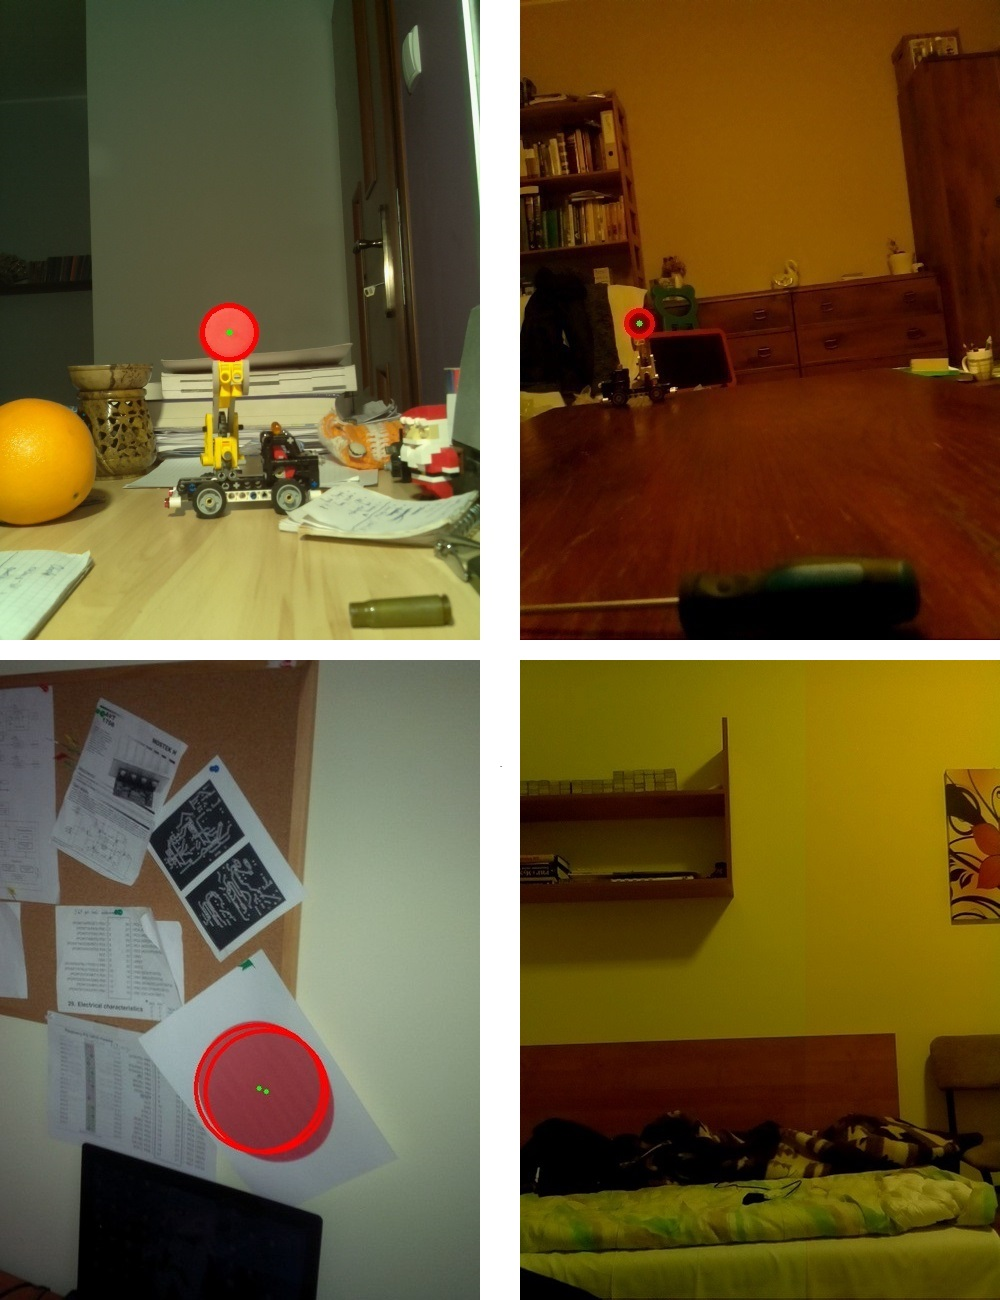
\includegraphics[scale=0.6]{imgs/circles.jpg}
\caption[Przykładowe efekty końcowe algorytmu wykrywającego okręgi.]\small{Ilustracja przedstawia trzy zdjęcia z czerwonymi obiektami wykonane w zróżnicowanym oświetleniu oraz jedno zdjęcie nie posiadające pożądanego obiektu, jednak przekolorowane sztucznym oświetleniem mogącym teoretycznie zmylić algorytm.}
\label{przyklady}
\end{center}
\end{figure}
